% Options for packages loaded elsewhere
\PassOptionsToPackage{unicode}{hyperref}
\PassOptionsToPackage{hyphens}{url}
%
\documentclass[
  12pt,
]{book}
\usepackage{lmodern}
\usepackage{setspace}
\usepackage{amsmath}
\usepackage{ifxetex,ifluatex}
\ifnum 0\ifxetex 1\fi\ifluatex 1\fi=0 % if pdftex
  \usepackage[T1]{fontenc}
  \usepackage[utf8]{inputenc}
  \usepackage{textcomp} % provide euro and other symbols
  \usepackage{amssymb}
\else % if luatex or xetex
  \usepackage{unicode-math}
  \defaultfontfeatures{Scale=MatchLowercase}
  \defaultfontfeatures[\rmfamily]{Ligatures=TeX,Scale=1}
\fi
% Use upquote if available, for straight quotes in verbatim environments
\IfFileExists{upquote.sty}{\usepackage{upquote}}{}
\IfFileExists{microtype.sty}{% use microtype if available
  \usepackage[]{microtype}
  \UseMicrotypeSet[protrusion]{basicmath} % disable protrusion for tt fonts
}{}
\makeatletter
\@ifundefined{KOMAClassName}{% if non-KOMA class
  \IfFileExists{parskip.sty}{%
    \usepackage{parskip}
  }{% else
    \setlength{\parindent}{0pt}
    \setlength{\parskip}{6pt plus 2pt minus 1pt}}
}{% if KOMA class
  \KOMAoptions{parskip=half}}
\makeatother
\usepackage{xcolor}
\IfFileExists{xurl.sty}{\usepackage{xurl}}{} % add URL line breaks if available
\IfFileExists{bookmark.sty}{\usepackage{bookmark}}{\usepackage{hyperref}}
\hypersetup{
  pdftitle={Observatorio de Cohesión Social},
  hidelinks,
  pdfcreator={LaTeX via pandoc}}
\urlstyle{same} % disable monospaced font for URLs
\usepackage[left=4cm, right=3cm, top=2.5cm, bottom=2.5cm]{geometry}
\usepackage{longtable,booktabs}
% Correct order of tables after \paragraph or \subparagraph
\usepackage{etoolbox}
\makeatletter
\patchcmd\longtable{\par}{\if@noskipsec\mbox{}\fi\par}{}{}
\makeatother
% Allow footnotes in longtable head/foot
\IfFileExists{footnotehyper.sty}{\usepackage{footnotehyper}}{\usepackage{footnote}}
\makesavenoteenv{longtable}
\usepackage{graphicx}
\makeatletter
\def\maxwidth{\ifdim\Gin@nat@width>\linewidth\linewidth\else\Gin@nat@width\fi}
\def\maxheight{\ifdim\Gin@nat@height>\textheight\textheight\else\Gin@nat@height\fi}
\makeatother
% Scale images if necessary, so that they will not overflow the page
% margins by default, and it is still possible to overwrite the defaults
% using explicit options in \includegraphics[width, height, ...]{}
\setkeys{Gin}{width=\maxwidth,height=\maxheight,keepaspectratio}
% Set default figure placement to htbp
\makeatletter
\def\fps@figure{htbp}
\makeatother
\setlength{\emergencystretch}{3em} % prevent overfull lines
\providecommand{\tightlist}{%
  \setlength{\itemsep}{0pt}\setlength{\parskip}{0pt}}
\setcounter{secnumdepth}{5}
\usepackage[utf8]{inputenc}
\usepackage[spanish]{babel}
\usepackage{geometry}
\geometry{letterpaper,left=2cm,top=2cm, right=2cm}
\usepackage{times}           
\usepackage{caption}
\captionsetup[figure, table]{labelfont={bf},labelformat={default},labelsep=period}
\usepackage{graphicx}
\usepackage{float}
\usepackage{booktabs}
\usepackage{longtable}
\usepackage{array}
\usepackage{multirow}
\usepackage{wrapfig}
\usepackage{float}
\usepackage{colortbl}
\usepackage{xcolor}
\usepackage{pdflscape}
\usepackage{tabu}
\usepackage{threeparttable}
\usepackage{pdfpages} %para pdf portada
\usepackage{fancyhdr} %headers

% fuente: https://stackoverflow.com/questions/45963505/coverpage-and-copyright-notice-before-title-in-r-bookdown
\let\oldmaketitle\maketitle 
\AtBeginDocument{\let\maketitle\relax}




\pagestyle{fancy}
\fancyhf{}
\fancyhead[R]{\emph{\nouppercase{\rightmark}}}
\fancyhead[L]{\emph{\nouppercase{\thepage}}}
% \fancyfoot[CE,CO]{\leftmark}
% \fancyfoot[LE,RO]{\thepage}

\renewcommand{\headrulewidth}{1pt}
% \renewcommand{\footrulewidth}{1pt}

\ifluatex
  \usepackage{selnolig}  % disable illegal ligatures
\fi
\usepackage[]{natbib}
\bibliographystyle{apalike}

\title{Observatorio de Cohesión Social}
\usepackage{etoolbox}
\makeatletter
\providecommand{\subtitle}[1]{% add subtitle to \maketitle
  \apptocmd{\@title}{\par {\large #1 \par}}{}{}
}
\makeatother
\subtitle{Experiencias internacional de monitoreo de la cohesión}
\author{}
\date{\vspace{-2.5em}2020-12-03}

\begin{document}
\maketitle

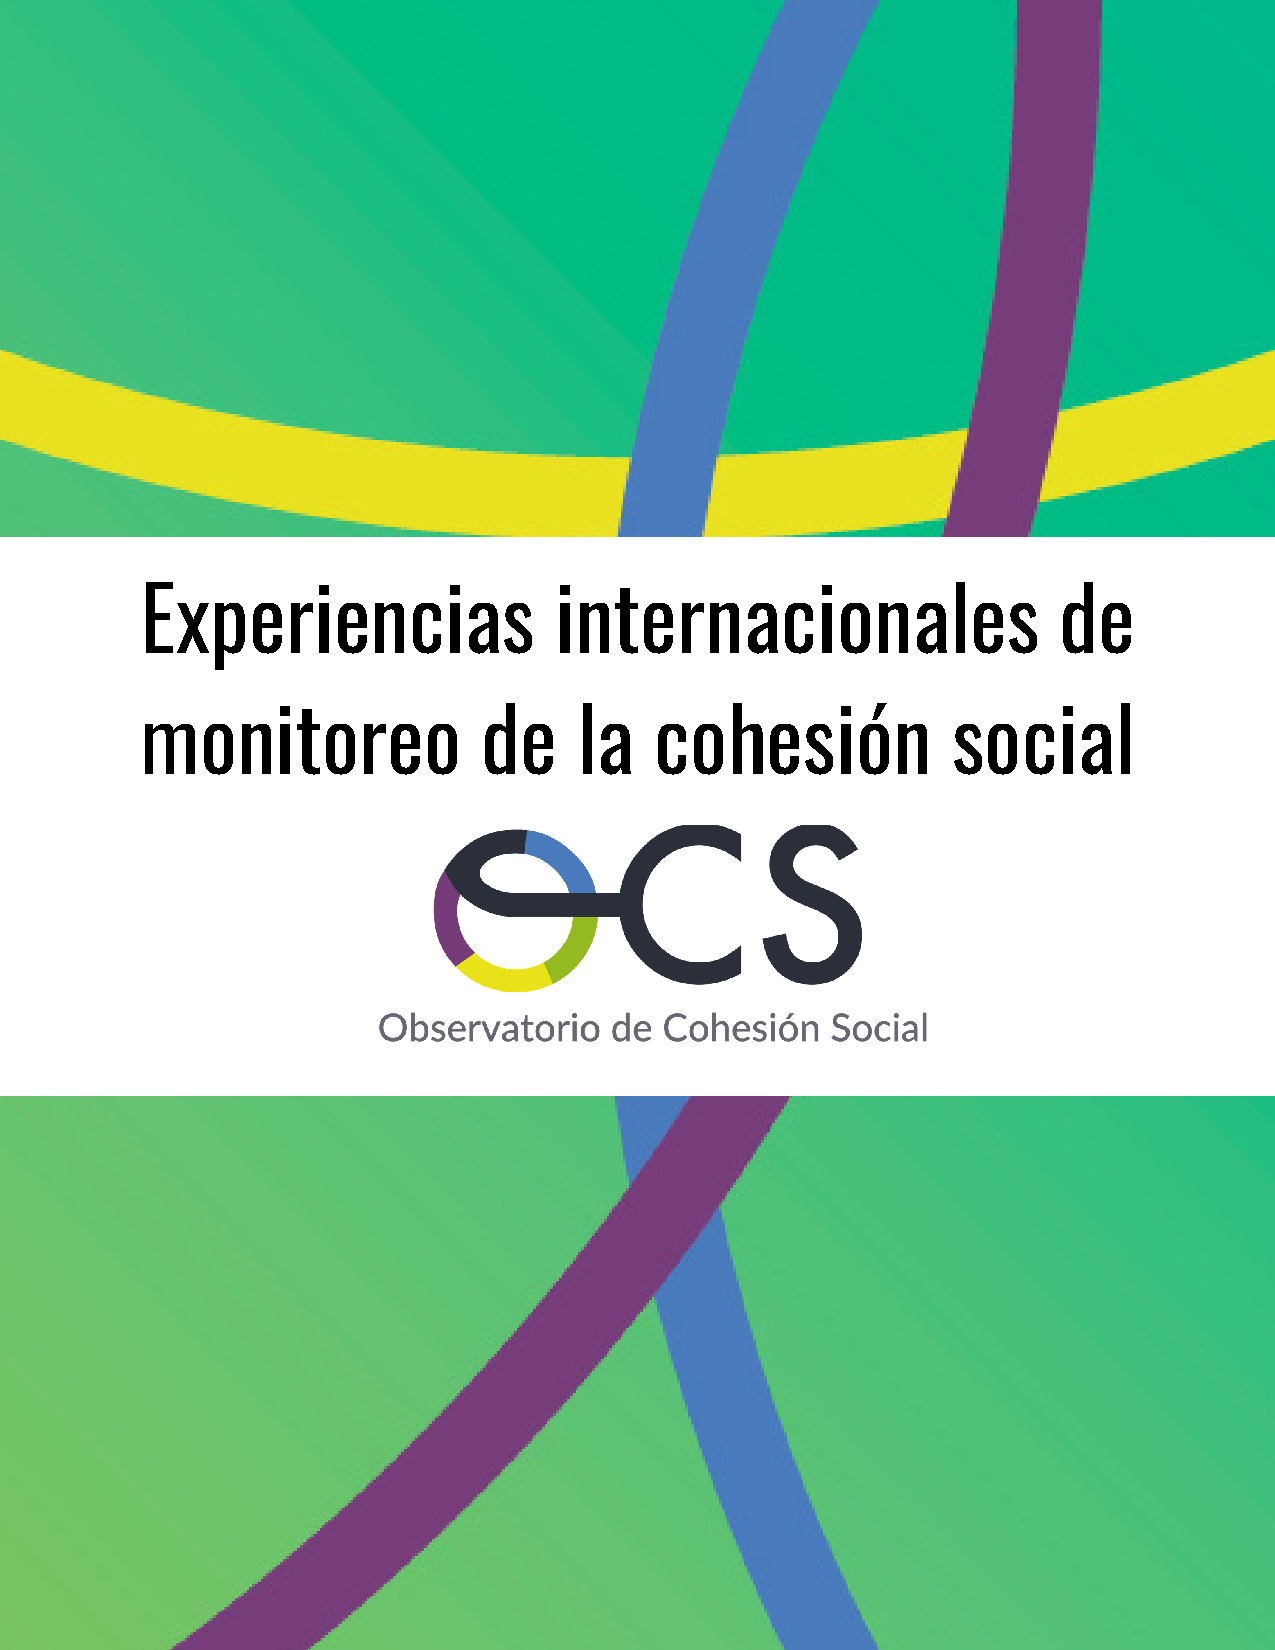
\includepdf[pages={1},scale=1.0]{inputs/frontpage.pdf}	

{
\setcounter{tocdepth}{1}
\tableofcontents
}
\listoftables
\listoffigures
\setstretch{1.5}
\hypertarget{introducciuxf3n}{%
\chapter{Introducción}\label{introducciuxf3n}}

Este reporte es un insumo para la creación del Observatorio de Cohesión
Social (OCS) del Centro de Estudios de Conflicto y Cohesión Social
(COES) que tiene como objetivo aumentar y centralizar la disponibilidad
de datos sobre cohesión social y ponerlos a disposición de la comunidad
académica nacional e internacional, la ciudadanía y los hacedores de
políticas públicas. Los datos e indicadores permitirán visualizar el
estado y trayectoria de la cohesión social para diversos países, con
especial énfasis en Chile.

Particularmente, el primer objetivo específico (recolectar datos e
indicadores internacionales sobre cohesión social, incluyendo su
adecuada documentación) hace necesaria la revisión de experiencias
internacionales que busquen monitorear la cohesión social en otros
contextos.

Como punto de partida de este esfuerzo por definir y operacionalizar la
cohesión social para el OCS es necesario considerar algunos trabajos de
carácter teórico que existen en Latino América. Uno de estos casos es el
trabajo realizado por la CEPAL \citep{ottone2007cohesion} una respuesta a los
problemas que afectan al continente, a saber, los altos índices de
pobreza, desigualdad y diversas formas de discriminación y exclusión. La
cohesión social en este caso está estrechamente vinculada a los valores
democráticos y el respeto al estado de derecho. Así, la cohesión social
tendría dos vertientes principales. Por un lado referiría a la capacidad
de los mecanismos instituidos de inclusión social (sistema educacional,
protección social, titularidad de derecho, etc.) como a los
comportamientos y valores de los sujetos que conforman la sociedad
(sentido de pertenencia, capital social, confianza en las instituciones,
solidaridad, etc.)

Otros de los casos destacados es el libro editado por Eugenio Tironi
``Redes, Estados y Mercados: soportes de la cohesión social en América
Latina''(2008) , en cuya introducción se entregan principios
orientadores y una definición de cohesión social
\citep{tironibarrios_Redes_2008} . Señalan que el concepto de cohesión social
es tanto descriptivo, por señalar lo que une a la sociedad, como
normativo por ponerla a la altura de los ideales que son propios de la
democracia. Una sociedad cohesionada no es una sociedad cerrada en torno
a determinados valores, sino la que permite que los sujetos se
relacionen en torno a principios de justicia que al ser respetado dan
fundamento al actuar cooperativo. Por eso, desde esta perspectiva el
concepto supone un sentido de pertenencia moral y sujeción a reglas al
estilo durkhemiano que son compatibilizados con la autonomía individual
para las sociedades modernas. Sin embargo, la conciencia moral podría
incluir elementos como la misma autonomía individual, la diferencia y la
diversidad como principios orientadores.

La revisión de experiencias internacionales en el monitoreo de cohesión
social tiene cuatro focos centrales. En primer lugar, conocer en mayor
detalle la estructura organizacional y objetivos de los proyectos
existentes actualmente. En segundo lugar, revisar las definiciones
conceptuales de cohesión social para entregar un marco general en el
cuál focalizar la búsqueda de datos para el caso chileno. El tercer foco
es la operacionalización que estas experiencias realizan del concepto
para identificar indicadores a considerar en el OCS. Finalmente, cada
revisión de las experiencias internacionales se concluye con un listado
de referencias comentadas en donde se puede encontrar documentos de
trabajo o aplicaciones de los datos levantados por cada uno de los
proyectos.

La selección de iniciativas internacionales buscó ser representativa
geográficamente dado que las perspectivas sobre la cohesión social tiene
un arraigo en los atributos socioculturales en los que estos se
desarrollan: vínculos sociales o capital social en Estados Unidos por
ejemplo o ampliación del Estado de Bienestar a grupos excluidos en
Europa.

Por esto se ha seleccionado el Scalon-Monash Index of Social Cohesión de
Australia, el Social Cohesión Radar alemán con alcance internacional, el
trabajo teórico Civic Engagement and Social Cohesion Report de los
Estados Unidos, el clásico trabajo de Jenson \citetext{\citeyear{jenson1998mapping}; \citeyear{jenson2010defining}} Mapping Social Cohesion en Canadá y el proyecto
ECOsociAL que comprendió a siete ciudades de Latinoamérica.

Se espera que con este insumo se pueda avanzar en la concreción del
objetivo específico 1 del proyecto del observatorio, que requiere de un
análisis de la disponibilidad de indicadores internacionales de cohesión
social a partir de conocer qué es lo que se ha considerado en otras
iniciativas.

\hypertarget{mapping-social-cohesion}{%
\chapter{Mapping Social Cohesion}\label{mapping-social-cohesion}}

\hypertarget{descripciuxf3n-general}{%
\section{Descripción General}\label{descripciuxf3n-general}}

El trabajo de \citet{jenson1998mapping} en Canadá es uno de los trabajos
pioneros que trató de dar orden a las discusiones sobre cohesión social.
Se reconoce que a fines del siglo XX los organismos gubernamentales y no
gubernamentales tenían una gran preocupación por el tema, pero no
existía una definición clara de lo que implicaba y la diferencia que
existía con otros conceptos asociados.

El trabajo de Jenson nace de la Mesa de trabajo del Canadian Policy
Research Network ``Mapping Social Cohesion" en diciembre de 1997. El
objetivo fue identificar la literatura emergente en el tema y definir
una agenda de investigación para hacer de estas ideas fundamentales una
forma más operacional de aproximarse al problema. El estudio revisa
analíticamente los orígenes del debate en la tradición sociológica hasta
los conceptos más actuales, incluyendo el estado del arte en Canadá.
Jenson señala textualmente que la ``clarificación es el objetivo primario
de este paper'' (1998: 2).

El trabajo fue financiado por Canadian Heritage, el Department of
Justice Canada y The Kahanoff Foundation Nonprofit Sector Research
Initiative.

\hypertarget{concepto-de-cohesiuxf3n-social}{%
\section{Concepto de Cohesión Social}\label{concepto-de-cohesiuxf3n-social}}

La conceptualización de \citet{jenson1998mapping} ha sido un recurso de suma
importancia para trabajos posteriores como el Scalon-Monash Index
australiano que lo utilizan como punto de partida. Para Jenson (1998),
la cohesión social es más un proceso que un estado o condición,
involucrando un sentido de compromiso, y deseo o capacidad de vivir
juntos en armonía.

La revisión conceptual del autor lo lleva a plantear que la literatura
ha reconocido a la cohesión social como una característica de la
sociedad y no de los individuos. El concepto de cohesión social es un
concepto con historia, partiendo de esta premisa es que
\citet{jenson2010defining} plantea que han existido tres familias vinculadas al
concepto con diferences aplicaciones empíricas.

La primera vincula la cohesión social a la noción de inclusión social. A
comienzo de los '80 la OCDE decidió revisar el concepto de cohesión
social en orden a hacerlo compatible con la restructuración económica de
los países miembros y a la vez sustentable en el tiempo. En este uso, se
desprendía que la OCDE estaba homologando cohesión social con
estabilidad social. Ya a comienzos del siglo XXI la UE orientaba sus
políticas sociales en la misma dirección y definía el desarrollo
económico y la cohesión social como objetivos principales. El Council of
Europe (organismo de la Unión Europea) señalaba explícitamente: \emph{"Social
cohesion, as defined by the Directorate General of Social Cohesion of
the Council of Europe, is a concept that includes values and principles
which aim to ensure that all citizens, without discrimination and on an
equal footing, have access to fundamental social and economic rights}``.
Se debe considerar que en esta conceptualización se tomó cuidado en
sugerir que la integración no implicaba necesariamente formas
tradicionales de integración social, siendo un concepto para una
sociedad abierta y multicultural. No obstante, \citet{jenson2010defining}
agrega que realmente no se estaba entregando una conceptualización clara
de lo que significaba cohesión social: ``it does not define social
cohesion as such but seeks to identify some of the factors in social
cohesion \ldots{}'' (citado por Jenson, 2010:5)

La segunda línea de conceptualización de la cohesión social lo hace en
relación a capital social o, incluso, como sinónimos. Para esta
tradición el capital social es la herramienta práctica para lograr la
cohesión social. El capital social no tan solo entrega recursos a los
invididuos, como acceso a servicios especiales a menor costo o para que
alguien cuide al hijo de una madre que debe ir a trabajar, sino que
produce un bien colectivo al tener sociedades más saludables. A esta
conceptualización liderada por Putnam, le siguieron una serie de
críticas sobre su caracter positivo y si realmente era social
considerando su enfoque focalizado en el individuo. Esto produjo el
refinamiento del concepto introduciendose los conceptos de capital
social bridging, bonding y linking.

Y finalmente, una tercera familia de estudios se focaliza en las
instituciones y la gobernanza liderada principalmente por el Banco
Mundial. Esta definición se superpone a las dos anteriores, pero toma un
caracter distinto. Señalan que los resultados económicos dependen de
instituciones efectivas, y esta a su vez de la cohesión social. Por lo
tanto, construir cohesión social es una tarea vital para el desarrollo.
El desafío está puesto en la inclusión de las personas en la provisión
de servicios públicos de forma equitativa y eficiente.

Si bien \citet{jenson2010defining} no entrega una definición propia de la
cohesión social, sino que una revisión del estado del arte en la
materia, la Social Cohesion Network reemplaza su definición de cohesión
social basada en valores por una más funcionalista fijada en las
conductas: ``la cohesión social está basada en la disposición de los
individuos a cooperar y trabajar en todos los niveles de la sociedad
para lograr metas comunes'' \citep{Jeannote2003}

La ventaja de esta definición y que la ha llevado a ser un referente
para posteriores experiencias en todo el mundo es que se focaliza
claramente en los resultados de la cohesión social y en el conjunto de
indicadores para medir el stock de cohesión social en la sociedad (
trabajar juntos, metas colectivas, cooperación, etc.). La tarea se
simplifica si consideramos desde la definición la igualdad de
oportunidades, las metas compartidas y valores.

\hypertarget{operacionalizaciuxf3n}{%
\section{Operacionalización}\label{operacionalizaciuxf3n}}

\begin{figure}[H]

{\centering 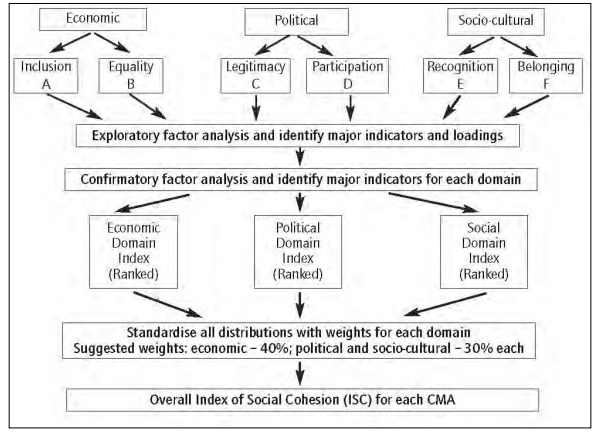
\includegraphics[width=0.75\linewidth]{inputs/images/mapping} 

}

\caption{Operacionalización de Mapping Social Cohesion}\label{fig:mapping}
\end{figure}

El concepto de cohesión social es operacionalizado inicialmente en 5
dimensiones.

\begin{enumerate}
\def\labelenumi{\arabic{enumi}.}
\item
  Pertenencia/aislamiento: esta dimensión es más o menos compartida
  por toda la literatura, y señala el grado en que los sujetos
  comparten valores e identidades colectivas. Valores compartidos
  permiten desarrollan un sentido de pertenencia y a la vez generar un
  sentido de comunidad.
\item
  Inclusión/exclusión: esta dimensión tiene un carácter institucional
  y en el mercado en particular como elemento central de la
  modernidad.
\item
  Participación/no-involucramiento: la cohesión social requiere
  involucramiento de parte de los sujetos. El desencantamiento con la
  política pondría en riesgo la cohesión social y obliga también a los
  gobiernos a fortalecer el tercer sector.
\item
  Reconocimiento/rechazo: se parte de la idea de que las sociedades
  modernas son pluralistas en su sistema de valores. El pluralismo es
  un bien y la tolerancia una meta. El rechazo, la intolerancia y
  excesivos esfuerzos por lograr la unanimidad irían contra la idea de
  reconocimiento de la diversidad.
\item
  Legitimidad/ilegitimidad: se señala que la intermediación necesaria
  para vivir con los conflictos de valores no depende de los sujetos,
  sino que es producto de las instituciones. Por lo tanto, en última
  instancia la cohesión social depende de la legitimidad que tienen
  las instituciones públicas y privadas en asegurar la cohesión
  social.
\end{enumerate}

Con esto en mente, \citet{jenson2010defining} plantea tres set de indicadores.
Un primer set de indicadores (1 - 5) corresponde a mediciones de
disparidades sociales, y las brechas indicarías acceso desigual a
recursos económicos y a servicios sociales básicos.

\begin{enumerate}
\def\labelenumi{\arabic{enumi}.}
\item
  Cohesión social como inclusión social relacionada al acceso de
  recursos financieros:

  \begin{itemize}
  \item
    Coeficiente de Ginni
  \item
    Mediciones de ingresos
  \item
    Mediciones de pobreza (población viviendo con menos de 1 dolar,
    población viviendo con menos de 2 dólares y población bajo la
    línea de pobreza).
  \end{itemize}
\item
  Cohesión social como inclusión social relacionada la actividad
  económica:

  \begin{itemize}
  \item
    Tasa de empleo (juvenil, femenina, minorías e inmigrantes)
  \item
    Empleo en economía informal, como porcentaje del empleo total
  \end{itemize}
\item
  Cohesión social como inclusión social relacionada con el acceso a
  educación y capital humano:

  \begin{itemize}
  \item
    Tasa de alfabetización (total, hombres y mujeres)
  \item
    Porcentaje de población sobre 15 años que no ha completado
    educación primaria (total, hombres y mujeres)
  \item
    Porcentaje de población sobre 20 años que no ha completado
    educación secundaria (total, hombres y mujeres)
  \item
    Porcentaje de niños en edad de educación secundaria matriculados
    en educación secundaria
  \item
    Porcentaje de población entre 18 y 24 años en educación
    terciaria
  \end{itemize}
\item
  Cohesión social como inclusión social relacionada con el acceso a la
  salud:

  \begin{itemize}
  \item
    Esperanza de vida al nacer (en años)
  \item
    Mortalidad infantil (por mil nacidos vivimos)
  \item
    Mortalidad bajo 5 años (por mil)
  \item
    Nacidos atendidos por equipo medido (porcentaje del total para
    toda la población y para las minorías)
  \end{itemize}
\item
  Cohesión social como inclusión social relacionada con el acceso a
  tecnología:

  \begin{itemize}
  \tightlist
  \item
    Porcentaje de hogares con internet de banda ancha
  \end{itemize}

  El segundo tipo de indicadores corresponden a medidas de
  homogeneidad cultural y étnicas vinculadas a la dimensión de
  diversidad de la cohesión social. Más diversidad es considerado para
  Jenson (2010) como un indicador de menos cohesión social.
\item
  Cohesión social como homogeneidad cultural y étnica

  \begin{itemize}
  \item
    Porcentaje de extranjeros en la población
  \item
    Fraccionalización étnica - índice que mide la probabilidad de
    que dos personas seleccionadas aleatoriamente pertenezcan al
    mismo grupo etnolinguístico
  \end{itemize}

  El tercer y último grupo de indicadores (7 - 8) corresponde a las
  dimensiones de pertenencia y participación.
\item
  Cohesión social como confianza

  \begin{itemize}
  \tightlist
  \item
    Preguntas sobre confianza desde encuestas de opinión pública. El
    autor plantea explícitamente la encuesta mundial de valores
  \end{itemize}
\item
  Cohesión social como participación y solidaridad

  \begin{itemize}
  \item
    Participación electoral como porcentaje de electores posibles
    que participan en elecciones nacionales
  \item
    Tasa de participación en asociaciones voluntarias. Nuevamente se
    hace referencia a la encuesta mundial de valores.
  \item
    Caridad. Porcentaje de personas que realizan donaciones.
  \end{itemize}
\end{enumerate}

\hypertarget{referencias}{%
\section{Referencias}\label{referencias}}

\begin{enumerate}
\def\labelenumi{\arabic{enumi}.}
\item
  Jeannotte, M. (2003). Social Cohesion: Insights From Canadian
  Research. Presented at the Conference on Social Cohesion, Hong Kong.

  En esta presentación la autora resume el trabajo de Jenson y la
  influencia que este ha tenido en la conceptualización de la cohesión
  social. Asimismo, es importante destacar que lo complementa los trabajos
  de Bernard en Canadá.
\item
  Jenson, J. (1998). Mapping social cohesion: The state of Canadian
  research (No.~F03). Ottawa: CPRN.

  Es el trabajo principal de desarrollo teórico de Jenson. Con este informe el concretiza el encargo de dar un panorama general de las conceptualizaciones de cohesión social
\item
  Jenson, J. (2010). Defining and Measuring Social Cohesion. Londres:
  Commonwealth Secretariat.

  En este libro, el autor actualiza la conceptualización de cohesión social y desarrolla el conjunto de indicadores para medirla que han sido incluidos en este informe
\item
  Jenson, J., \& Saint-Martin, D. (2003). New routes to social
  cohesion? Citizenship and the social investment state. Canadian
  Journal of Sociology, 28(1), 77--99.

  Este artículo es un ejemplo de la aplicación del trabajo que ha desarrollado Jenson desde la Universidad de Montreal como investigadora. Aquí plantea la importancia de la consideracipon de la cohesión para el rediseño de la estructura de bienestar y de la inversión social que deben realizar las comunidades políticas.
\end{enumerate}

\hypertarget{scanlon-monash-index-of-social-cohesion}{%
\chapter{Scanlon-Monash Index of Social Cohesion}\label{scanlon-monash-index-of-social-cohesion}}

\hypertarget{descripciuxf3n-general-1}{%
\section{Descripción General}\label{descripciuxf3n-general-1}}

Este estudio ha sido realizado en Autralia 7 veces entre el 2007 y el
2014. La Fundación Scalon, responsable del estudio, tiene como fin desde
su creación en el 2001 contribuir a que Australia sea un país acogedor,
próspero y cohesivo.

En este marco, el estudio tiene por objetivo saber si en el futuro puede
ser sostenible la migración y la cohesión social que han caracterizado a
Australia desde la Segunda Guerra Mundial. De esta forma, el Monash
Institute for the Study of Global Movements y el Australian
Multicultural Foundation, con fondos de la Fundación Scanlon , encargó
el profesor Dr.~Andrew Markus \citep{markus_Attitudinal_2007, markus2013mapping}de la Monash University diseñar y dirigir una
medición de la cohesión social que sería repetida cada dos años. El
estudio fue conducido por el Melbourne-based Social Research Centre.

La cohesión social no es medida en abstracto, sino que se examina en el
contexto del impacto social de periodo prolongado de inmigración
significativa y sostenida. En los últimos años se ha profundizado con
encuestas comparadas en áreas de alto nivel de inmigración. Esto es de
relevancia, porque uno de los hallazgos más importantes del estudio ha
sido que la inmigración es un recurso de tensión social y debe ser
considerado por los estudios como los que realiza el COES. Estas
encuestas locales han sido realizadas el 2009, 2012, 2013 y se ha
planificado para el año 2015. Esto ha sido realizado desde el 2013 con
fondos del gobierno federal, lo que demuestra un trabajo que ha
involucrado a organizaciones sin fines de lucro, academia y ahora al
gobierno.

El proyecto tiene como objetivo explícito estimular a la discusión
basada en evidencia sobre el crecimiento de la población australiana y
la relación entre inmigración y cohesión social. Para esto, el
componente principal es la disposición de un sitio web con la
información, de la misma forma como se busca realizar con el
Observatorio de Cohesión Social. En este caso el sitio se denomina
``Mapping Australia's Population''.

El sitio entrega información para la discusión de políticas públicas
sobre inmigración y cohesión social en base a los datos de la encuesta.
Aunque existe un repositorio con encuestas que han sido conducidas en
Australia y con una regular actualización.

En cuando al diseño muestral, el 2014 se utilizaron dos muestras.
Primero, el tradicional muestreo bietápico realizado desde la primera
versión del instrumento basado en el universo de adultos con línea
telefónica al que se le agregaron las personas con teléfono celular
(1.526). La segunda muestra de australianos con ambos padres
australianos es de internet (1.070), incorporando diseños
experimentales.

En cuanto a las características del instrumento, todos los años se han
aplicado los 18 indicadores del Índice Scalon-Monash de Cohesión Social.
La aplicación online es igual a la telefónica, pero adicionando 17
preguntas de identidad, diversidad cultural e integración. Para el 2014,
el cuestionario fue de 65 preguntas y una aplicación de 16.2 minutos de
duración promedio.

\hypertarget{concepto-de-cohesiuxf3n-social-1}{%
\section{Concepto de Cohesión Social}\label{concepto-de-cohesiuxf3n-social-1}}

El concepto que utilizan en el SMISC (Scanlon-Monash Index of Social
Cohesion) recoge una visión ecléctica de la tradición académica. Su
conceptualización ha estado principalmente influida por los trabajos de
los canadienses Paul Bernard y Jane Jenson que señalan que el objetivo
general de la cohesión social es que todos los ciudadanos puedan acceder
en iguales condiciones a los derechos económicos y sociales
fundamentales.

En el desarrollo del proyecto se reconoce la tradición que destaca la
importancia del papel que juegan el consenso y el conflicto en las
sociedades. El interés en este concepto ha sido alentado por los
procesos sociales generales como la globalización, el cambio económico y
la guerra contra el terrorismo en las últimas décadas. Sin embargo, la
creación de este índice se enfrenta al problema más común en la
conceptualización de teorizaciones acerca de la social: no hay acuerdo
en la definición del concepto.

Según los autores del índice, las definiciones actuales muchas veces son
intangibles, y refieren a una característica de un grupo o la
disposición de lo sujetos para participar y compartir objetivos. En este
marco, y en el intento de concretizar la conceptualización con un
enfoque ecléctico se llegó a la identificación de tres elementos
comunes: la cohesión social es una visión compartida, una propiedad
grupal y un proceso.

La visión compartida refiere a que los investigadores reconocen que la
cohesión social requiere de valores universales, respeto mutuo y
aspiraciones comunes o identidades compartidas por los miembros.
Asimismo, hay acuerdo en que este constructo es una propiedad de los
grupos o comunidades en los que existe esa visión compartida sobre metas
y responsabilidades. Finalmente, la cohesión social es comunmente vista
como un continuo y un proceso sin fin de búsqueda de la armonía social y
no un resultado como se podría pensar.

Por otro lado, la diferencia en las definiciones de cohesión social
están puestas fuertemente en los factores que impactan sobre el proceso
de armonía de los grupos o comunidades. Esto último debe ser considerado
por el OCS para identificar aquellas variables que permitirán segmentar
los distintos indicadores de cohesión social buscando explicar la
variabilidad entre grupos y países. Los factores claves que reconocen en
el SMISC son económicos, políticos y socioculturales. En cuanto a los
factores económicos, se reconocen los niveles de desempleo y pobreza,
distribución de ingreso, migraciones, salud, satisfacción con la vida y
sentido de seguridad, y la responsabilidad del gobierno por la pobreza y
la desigualdad. En lo político, los factores que influyen sobre la
cohesión social están relacionados al nivel de participación política e
involucramiento social, incluyendo el voluntariado, el desarrollo de
capital social, y las normas y confianza social que facilitan la
cooperación en los grupos o comunidades. Finalmente, a nivel
sociocultural se considera el consenso y la divergencia en torno a temas
de significación nacional y local.

En resumen, la definición que el SMISC entrega sobre cohesión social es
la disposición que tienes lo miembros de una sociedad para cooperar con
cada uno de los demás para la sobrevivencia y la prosperidad. En virtud
de esto, el SMISC cubre cinco dominios de la cohesión social:

\begin{enumerate}
\def\labelenumi{\arabic{enumi}.}
\item
  Pertenencia: esta dimensión comprende los valores que comparte la
  población, la identificación con el país (Australia) y la confianza.
\item
  Valoración: comprende la satisfacción con la situación económica,
  satisfacción con la vida, felicidad y expectativas sobre el futuro.
\item
  Justicia social y equidad: visión sobre el adecuado apoyo a las
  personas de bajos ingresos, la brecha entre ricos y pobres, el país
  como una tierra de oportunidades y confianza en el gobierno.
\item
  Participación (política): trabajo voluntario, actividad e
  involucramiento político.
\item
  Aceptación, rechazo y legitimidad: experiencia de discriminación,
  actitudes hacia las minorías y \emph{newcomers}.
\end{enumerate}

\hypertarget{operacionalizaciuxf3n-1}{%
\section{Operacionalización}\label{operacionalizaciuxf3n-1}}

Uno de los elementos característicos de la iniciativa australiana es el
diseño de un índice de cohesión social el que ha sido medido en cada una
de las versiones del estudio.

El Scanlon-Monash Index de Cohesión Social esta compuesto por 5
dimensiones que resumen los dominions del concepto.

\begin{figure}[H]

{\centering 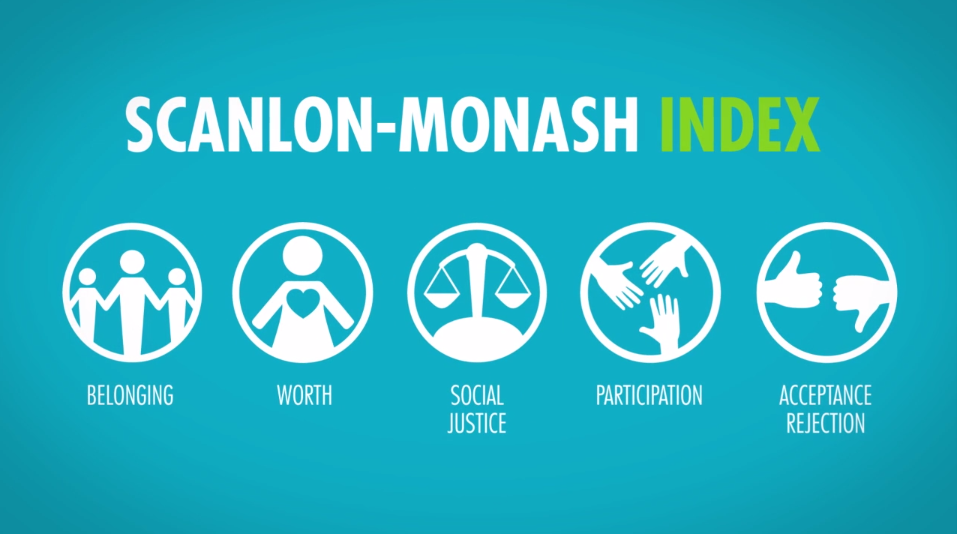
\includegraphics[width=0.75\linewidth]{inputs/images/scalon} 

}

\caption{Operacionalización del Índice de Cohesión Social}\label{fig:scalon}
\end{figure}

La primera dimensión corresponde al \textbf{sentido de pertenencia} que
incluye preguntas generales sobre el sentido de pertenencia, sentido de
orgullo y la importancia de mantener la cultura y forma de vida de los
australianos. Los dos primeros medidos en una escala de cuatro puntos
desde To a great extent a Not at all. La importancia de la cultura y
forma de vida utiliza una escala de acuerdo de 4 puntos.

La segunda dimensión es la \textbf{valoración} compuesta por un indicador de
satisfacción con la situación financiera y felicidad en los últimos
años.

La tercera dimensión es la \textbf{equidad y justicia social} medido con el
nivel de acuerdo acerca de que Australia es una tierra de oportunidades
en donde el trabajo duro entrega una mejor vida; el grado de acuerdo con
que existe una gran diferencia entre altos ingresos y bajos ingresos;
que las personas con bajos ingresos reciben suficiente apoyo; y que el
gobierno federal hace las cosas correctas por las personas.

La cuarta dimensión es la \textbf{participación política} medido a través de
un índice que combina distintas formas de participación: votar en
elecciones, firmar una petición, contacto con miembros del parlamento,
unirse a un boycot de algún producto comercial y asistir a una protesta,
marcha o demostración.

Finalmente, el índice incluye una dimensión de \textbf{aceptación y rechazo}
compuesta de indicadores de experiencia de discriminación en base a
color de piel, etnia o religión; pesimismo sobre el futuro preguntado a
través de si cree que en 3 años su vida en Australia estará peor, igual
o mejor; si cree que el gobierno australiano debe dar asistencia para
que las minorías étnicas mantengan sus costumbres y tradiciones; y si
cree que aceptar inmigrantes de muchos países hace a Australia más
fuerte. \citep{colic-peisker_Social_2015}

En conjunto con las preguntas para la construcción del índice de
cohesión social, las diferentes versiones del estudio han incluido otras
mediciones complementarias y un análisis particular de los indicadores
incluidos en el índice general. Para el año 2014 los indicadores
incluidos cubrían:

\begin{itemize}
\item
  Ranking de problemas más importantes hoy en día en el país a través
  de una pregunta abierta que busca determinar los temas que son más
  importantes para los australianos.
\item
  Experiencia de discriminación por piel, etnia o religión en los
  últimos doce meses. El 2014 incluyó una pregunta sobre la frecuencia
  en la que ocurrió y el lugar (barrio, trabajo, centro comercial,
  transporte público o evento deportivo). La percepción sobre el
  barrio es profundizada en esta sección en base a una serie de
  indicadores sobre percepción de seguridad.
\item
  Confianza interpersonal y trabajo voluntario en los últimos doce
  meses.
\item
  Democracia a través de preguntas sobre la opinión del rol del
  gobierno. El grado de acuerdo con que el gobierno realiza las cosas
  correctas para los australianos; preferencias por diferentes
  sistemas políticos y por la democracia en específico. En esta
  sección se incluye la confianza en distintas instituciones.
\item
  Policía y sistema legal. Confianza en la policía y sistema legal,
  contacto con la policía, percepción del trabajo de la policía
  (honestidad, trato equitativo y profesionalismo), satisfacción con
  la respuesta.
\item
  Inmigración es el tema más importante del instrumento. En el informe
  del 2014 se reporta el nivel de conformidad con el actual nivel de
  inmigración y su proyección.
\item
  Búsqueda de asilo y refugiados ocupan una sección especial en el
  informe. Se explora en el nivel de conocimiento sobre el fenómeno,
  las razones de esto y si son considerados por la población como un
  fenómeno de inmigración ilegal. Se pregunta en específico por
  aquellas personas que llegan al país en barco buscando asilo
  distinguiéndolos de aquellos refugiados por programas humanitarios.
  Uno de los aspectos más interesantes es que se le pregunta a la
  población qué hacer con la población que llega a través de barcos
  (postular a residencia permanente, temporal, enviar de vuelta o que
  el barco regrese).
\item
  Multiculturalismo y diferencia de valores. Se pregunta el grado de
  acuerdo con 5 frases sobre multiculturalismo (beneficio para el
  desarrollo económico, discurso de que los inmigrantes sean parte de
  la sociedad, debilita la forma de vida australiana, dar a los
  inmigrantes las mismas o más oportunidades que los nacidos en
  Australia y reducir los problemas de los inmigrantes.
\end{itemize}

\hypertarget{referencias-1}{%
\section{Referencias}\label{referencias-1}}

\begin{enumerate}
\def\labelenumi{\arabic{enumi}.}
\item
  Markus, A. \& Dharmalingam, A. (2014). Mapping Social Cohesion: The
  Scanlon Foundation surveys 2014.

  Este informe presenta los resultado de la encuesta de Scalon Foundation. En cada informe se resume la construcción del índice y las dimensiones que comprenden en su propuesta de operacionalización de la cohesión social.
\item
  Colic-Peisker, V. \& Robertson, S. (2015). Social change and
  community cohesion: an ethnographic study of two Melbourne suburbs.
  Ethnic and Racial Studies, 38(1), 75-91.

  Dado el importante énfasis local que ha tenido esta encuesta, ha
  generado problematizaciones que han sido cubiertas por otros
  investigadores como es el ejemplo de este estudio etnográfico. Los
  autores se plantean la pregunta de hasta qué punto comunidades
  etnoculturalmente diversas pueden ser cohesivas.
\item
  Markus, A., \& Dharmalingam, A. (2007). Attitudinal Divergence in a
  Melbourne Region of High Immigrant Concentration: A Case Study.
  People and Place, 15(4), 38-48.

  En este artículos los autores utilizan datos de la encuestas
  Scalon-Monash para comprender las actitudes hacia la inmmigración y
  la diversidad étnica en dos suburbios de Melbourne. Los resultados
  sugieren que existe un apoyo hacia la no-selección en la aplicación
  de políticas sociales en base a criterios étnicos, aunque hay cierto
  rechazo a la inmigración y algunos aspectos del multiculturalismo.
\end{enumerate}

\hypertarget{social-cohesion-radar}{%
\chapter{Social Cohesion Radar}\label{social-cohesion-radar}}

\hypertarget{descripciuxf3n-general-2}{%
\section{Descripción General}\label{descripciuxf3n-general-2}}

El Social Cohesion Radar (SCR) es un esfuerzo por aportar información al
debate público sobre cohesión social, un mejor entendimiento de los
cambios actuales y la proyección en el futuro. Su objetivo explícito es
proveer al público general de una buena visualización de conjunto de los
niveles y tendencias de la cohesión social tanto como una comprensión en
profundidad de sus determinantes y resultados.

El radar ha comparado la tendencia en la cohesión social de 34 países
entre 1989 y 2012. La encuesta ha incluido 27 países miembros de la
Unión Europea (sin Croacia) tanto como 7 naciones industrializadas de
occidente (Estados Unidos, Canadá, Noruega, Suiza, Israel, Australia y
Nueva Zelanda).

Actualmente se trabaja en la identificación de causas, efectos y futuras
tendencias. Esta es una iniciativa de Bertelsmann Stiftung en
cooperación con académicos de la Jacobs University Bremen.

Uno de los rasgos particulares del radar es que está hecho completamente
en base a datos secundarios, es decir se reutilizan otros datos
recopilados por los mismos u otros investigadores para medir cuestiones
similares en los países objetos de estudio. Se señala que la utilización
de datos secundarios tiene como ventaja que se realiza en base a datos
validados y confiables de encuesta de gran escala en diferentes países.
Dado que se reduce considerablemente los costos, hay un mayor alcance
del estudio. Y, finalmente, es posible realizan el estudio de forma
retrospectiva.

\hypertarget{concepto-de-cohesiuxf3n-social-2}{%
\section{Concepto de Cohesión Social}\label{concepto-de-cohesiuxf3n-social-2}}

La conceptualización del SCR no difiere en gran medida de la experiencia
australiana partiendo de la misma base de la incapacidad hasta ahora de
haber generado una conceptualización unívoca del concepto aunque si de
su multidimensionalidad.

En este proyecto, se identifican de la misma forma tres aspectos comunes
a las distintas definiciones de cohesión social. Al igual que SMISC la
cohesión social es un atributo del colectivo y no de los sujetos en
particular. También existe una gradualidad de la cohesión social, de tal
forma que las sociedades, ciudades, barrios o grupos pueden ser más o
menos cohesivos. Y, finalmente, los individuos pueden experimentar
distintos niveles de bienestar con distintos niveles de cohesión social.
Este último aspecto es un elemento no señalado explícitamente en la
definición utilizada por el SMISC y que plantearía que la cohesión
social no es un concepto positivo con valor en si mismo, sino que se
debe contextualizar.

La definición que ha elaborado el equipo del radar es que ``Una sociedad
cohesionada se caracteriza por relaciones sociales resilientes,
conexiones emocionales positivas entre los miembros y la comunidad y una
foco pronunciado en el bien común. Las relaciones sociales, en este
contexto, son la red horizontal que existe entre los individuos y los
grupos dentro de la sociedad. La conectividad refiere a los vínculos
positivos entre individuos y sus países e instituciones. Un foco en el
bien común finalmente, es reflejado en las acciones y actitudes de los
miembros de la sociedad que demuestran responsabilidad por otros y por
la comunidad como un todo. Estos son los tres aspectos central de la
cohesión'' \citep{dragolov2013social, delhey_Happier_2016}

\hypertarget{operacionalizaciuxf3n-2}{%
\section{Operacionalización}\label{operacionalizaciuxf3n-2}}

El concepto utilizado en el Radar de Cohesión Social esta compuesto por
tres dimensiones que a su vez se dividen en tres dimensiones cada una.
Estas dimensiones han sido evaluadas en cuatro periodos de tiempo
distinto con diferentes indicadores producto de la disponibilidad de
datos. Para cada subdimensiones se reportarán los indicadores utilizados
en el cuarto periodo de tiempo (2009-2012).

\begin{figure}[H]

{\centering 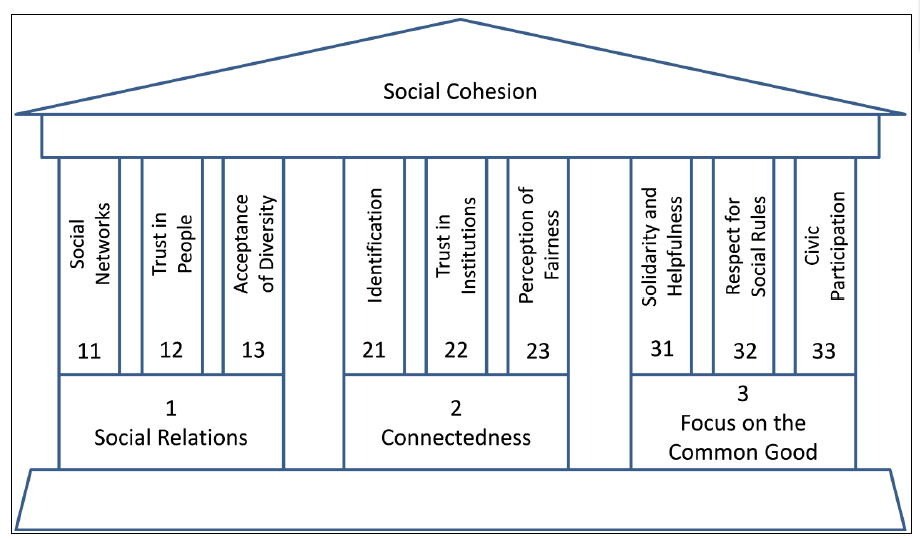
\includegraphics[width=0.75\linewidth]{inputs/images/radar} 

}

\caption{Operacionalización del Radar de Cohesión Social]}\label{fig:radar}
\end{figure}

Las relaciones sociales, en tanto redes horizontales que existen entre
los individuos y grupos de la sociedad, está compuesto por redes
sociales, confianza en las personas y aceptación de la diversidad. Una
sociedad cohesionada debería presentar fuertes redes sociales, alto
nivel de confianza en otros y considerar a individuos con diferentes
estilos de vida y valores como iguales.

\emph{Redes sociales}

\begin{itemize}
\item
  Count on to help
\item
  How much time during past week you felt lonely
\item
  Support if needed advice on serious personal or family matter
\item
  How often socially meet with friends, relatives or colleagues
\end{itemize}

\emph{Confianza en las personas}

\begin{itemize}
\item
  People try to be fair
\item
  Most of the time people helpful
\item
  People can be trusted
\end{itemize}

\emph{Aceptación de la diversidad}

\begin{itemize}
\item
  Country's culture undermined by immigrants
\item
  Rating of religious tension (high score, low tension)
\item
  City/area good place for: Racial/ethnic minorities
\item
  Rating of ethnic tension (high score, low tension)
\item
  City/area good place for: Gay or lesbian people
\item
  Gays and lesbians free to live life as they wish
\end{itemize}

La segunda dimensión de la cohesión es la conectividad entendida como
los vínculos entre individuos, su país y sus instituciones. A su vez,
esta dimensión está compuesta por tres subdimensiones: la
identificación, la confianza en las instituciones y percepción de
justicia. Un grupo altamente cohesionado debería tener una fuerte
conexión e identificación con él, alta confianza en las instituciones y
sentir que son tratados de forma justa. Los indicadores utilizados en el
cuarto periodo son:

\emph{Identificación}

\begin{itemize}
\item
  How attached to country
\item
  Ideally, would permanently move to another country
\end{itemize}

\emph{Confianza en las instituciones}

\begin{itemize}
\item
  Trust in parliament
\item
  Trust in political parties
\item
  Confidence in judicial system
\item
  Confidence in local police
\item
  Honesty of elections
\item
  Confidence in health care
\item
  Confidence in financial institutions
\end{itemize}

\emph{Percepción de justicia}

\begin{itemize}
\item
  To get ahead need to be corrupt
\item
  Corruption within businesses
\item
  Government should reduce differences in income levels
\item
  Corruption (high score, low corruption)
\item
  Tensions between the rich and the poor
\item
  I earn what I deserve
\item
  Pay about just for me
\end{itemize}

La tercera y última dimensión corresponde al foco en el bien común cuyas
tres subdimensiones son la solidaridad y amabilidad, respeto por las
normas sociales y participación cívica. En este caso, un grupo
cohesionado se caracteriza por que los miembros están preocupados por el
bienestar de unos y otros, respeto y aceptación de reglas y normas, y
participación en vida social y política. Los indicadores del cuarto
periodo de tiempo son:

\emph{Solidaridad y amabilidad}

\begin{itemize}
\item
  Helped a stranger
\item
  Unpaid voluntary work through community and social ser-vices
\item
  Donated money
\end{itemize}

\emph{Respeto por las normas sociales}

\begin{itemize}
\item
  How wrong to commit traffic offense
\item
  Size of shadow economy
\item
  Feel safe walking alone at night
\end{itemize}

\emph{Participación cívica}

\begin{itemize}
\item
  Worked in association or organisation
\item
  Signed a petition
\item
  Worn or displayed campaign badge/sticker
\item
  Interest in politics
\item
  Voiced opinion to public official
\item
  Volunteered time to organization
\item
  Voting turnout in elections or referenda
\end{itemize}

\hypertarget{referencias-2}{%
\section{Referencias}\label{referencias-2}}

\begin{enumerate}
\def\labelenumi{\arabic{enumi}.}
\item
  Bertelsmann-Foundation (2013). Social Cohesion Radar. Measuring
  Common Ground. An International Comparison of Social Cohesion.
  Gütersloh, Germany: Bertelsmann-Foundation.

  En este informe los autores presentan los principales resultados del
  índice de cohesión social para los distintos países en los que ha
  sido construido. También se incluye una breve conceptualización de
  lo que comprenden por cohesión social.
\item
  Bertelsmann-Foundation (2013). Social Cohesion Radar. Measuring
  Common Ground. Methods Report. Gütersloh, Germany:
  Bertelsmann-Foundation.

  En este informe se detallan los aspectos metodológicos del índice.
  Aquí se puede encontrar el detalle de los indicadores utilizados
  para cada medición y las fuentes de información.
\item
  Delhey, J., \& Dragolov, G. (2015). Happier together. Social cohesion
  and subjective wellbeing in Europe. International Journal of
  Psychology.

  Este artículo utiliza los datos del índice de cohesión social del
  radar para comprender cómo esta afecta al bienestar subjetivo para
  27 países de la Unión Europea. Los resultados sugieren que europeos
  en sociedades más cohesivas son más felices y saludables
  sicológicamente.
\end{enumerate}

\hypertarget{civic-engagement-and-social-cohesion-report}{%
\chapter{Civic Engagement and Social Cohesion Report}\label{civic-engagement-and-social-cohesion-report}}

\hypertarget{descripciuxf3n-general-3}{%
\section{Descripción General}\label{descripciuxf3n-general-3}}

La Corporacion para Servicios Nacionales y Comunales (CNCS en ingles)
destaca la importancia del involucramiento, cohesión social y capital
social para las grupos y sociedades, y trabaja en torno a estos tres
conceptos. No obstante, dado los objetivos de este reporte el análisis
se enfoca en el concepto de cohesión social, sin dejar de considerar la
relevancia y relación con los otros dos constructos.

Así, la CNCS encomendó que el Comité en Estadísticas Nacionales creara
un panel para identificar mediciones que puedan contribuir a mejorar el
entendimiento de los conceptos incorporados en este reporte y su rol en
explicar el funcionamiento de la sociedad.

El objetivo comisionado a este panel debía considerar los marcos
conceptuales, definiciones de conceptos claves, factibilidad y
especificaciones de indicadores relevantes, y la relación de estos
indicadores y la tendencias sociales. En este sentido, el panel evaluó
los méritos de las encuestas, los registros administrativos y datos no
gubernamentales. Uno de los estudios sobre capital social referentes
para el panel fue el Civic Engagement and Volunteer Supplements of
Current Population Survey (CPS), realizado por el U.S. Census Bureau.

La importancia de la recolección de datos y medición de los conceptos
del reporte que enfatiza el panel se base en la evidencia que los
conecta con resultados en dominios específicos como la salud, el crimen,
la educación, el empleo y la efectividad del gobierno; el valor de la
información descriptiva como insumos para comprender a la sociedad; y su
valor político y académico.

La relevancia de medir el capital social, involucramiento cívico y
cohesión social está también justificado en este caso desde las
políticas públicas. Se hace un resumen de los principales hallazgos de
la literatura: efecto sobre la prevalencia de cigarro e hipertensión; el
efecto del barrio sobre la seguridad y el crimen; efectos sobre la
resilencia y vulnerabilidad ante desastres naturales; efecto de la
inmigración y diversidad étnica sobre la cohesión social.

La proyecto fue auspiciado por la CNCS con recursos adicionales de la
National Conference on Citizenship (NCoC) y el U.S Office of Management
and Budget. Nathan Dietz (CNCS), Christopher Spera (CNCS), John
Bridgeland (NCoC), David Smith (NCoC) y Brian Harris-Kojetin (U.S.
Office of Management and Budget) definieron para el panel los objetivos
guía del estudio.

Un aspecto importante es que el estudio incorpora también prioridades de
investigación, desarrollo e implementación a partir de las conclusiones
del informe. Sin embargo, el foco principal del estudio es el rol del
sistema estadístico federal para mejorar la medición de capital social a
través de sus encuestas \citep{prewitt_Civic_2014}.

\hypertarget{concepto-de-cohesiuxf3n-social-3}{%
\section{Concepto de Cohesión Social}\label{concepto-de-cohesiuxf3n-social-3}}

El punto de partida del reporte es que el concepto de cohesión social se
diferencia de los conceptos de involucramiento civíco y capital social.
La cohesión social refiere a la extensión en la cual los grupos y
comunidades cooperan, se comunican para mejorar el entendimiento,
participan en actividades y organizaciones, y cooperan para responder a
los cambios. Nuevamente estamos frente a un concepto que se sitúa a
nivel de grupo y puede corresponder tanto a medios y fines, y no solo a
estos últimos. La cohesión social, a diferencia del involucramiento
cívico, refiere a las condiciones que hacen posible la acción o son
consecuencia de ella.

De forma similar a las demás iniciativas examinadas, el informe destaca
la dificultad de medir cohesión social, producto del número importante
de dimensiones y la complejidad asociada a cada una de ellos. Por
ejemplo, el sentido compartido de moralidad, valores y propósitos
comunes; niveles de orden social; extensión de la solidaridad creada por
la equidad de ingresos y riqueza; interacción social con y a través de
comunidades; y sentido de pertenencia.

Los autores citan a Forrest y Kearns para señalar que una sociedad sin
cohesión social debería ser una con un gran desorden social y conflicto,
valores morales no compartidos por las personas, extrema inequidad,
bajos niveles de interacción social entre y en las comunidades, además
de bajos niveles de pertenencia.

La escala espacial es una dimensión esencial del concepto de cohesión
social. Barrios, estados, u otros grupos podrían estar en conflicto con
otros mientras paralelamente demuestran una fuerte cohesión social
interna. En este sentido, es necesario especificar el nivel en el que se
está trabajando, cómo se forma la cohesión social y la función que está
ocupando en los distintos niveles de la familia a los países y todos los
niveles entre ellos.

Un elemento importante a considerar es que los autores del reporte
señalan que las actitudes y acciones de los individuos pueden unirlos o
separarlos en torno a ellas, por eso es que se deben considerar los
clivajes entre grupos opuestos que pueden ser cohesivos en torno a su
posición.

\hypertarget{operacionalizaciuxf3n-3}{%
\section{Operacionalización}\label{operacionalizaciuxf3n-3}}

La cohesión se plantea como una subdimensión de la medición propuesta de
capital social. En este caso se posiciona como un constructo
diferenciado a otros que suelen identificarse como parte de él. Las
otras dimensiones son integración social, equidad social, polarización
política, confianza en las instituciones, confianza interpersonal,
información, involucramiento político y no político. Sin embargo, dado
los objetivos de este informe se reporta a continuación la
operacionalización de la dimensión cohesión.

Si bien, los autores no llegan al nivel de plantear indicadores si
proponen variables y sus características (unidad de análisis, naturaleza
del fenómeno y forma de recolección). Para el caso de la cohesión son 8
las variables propuestas, todas posibles de recolectar mediante
encuestas:

\begin{itemize}
\item
  Frecuencia de interacción con familia/amigos: la unidad de análisis
  relevante en este caso es el individuo, es un fenómeno conductual
\item
  Ayuda de familia o amigos (redes de apoyo): la unidad de análisis
  relevante en este caso es el individuo, es un fenómeno conductual
\item
  Frecuencia de sentimiento de soledad: la unidad de análisis
  relevante en este caso es el individuo, es un fenómeno actitudinal
\item
  Participación en grupos de chat online: la unidad de análisis
  relevante en este caso es el individuo, es un fenómeno conductual
\item
  Vínculos intergrupales: la unidad de análisis relevante en este caso
  es el grupo, es un fenómeno conductual, actitudinal y que involucra
  características del entorno social.
\item
  Vínculos intragrupales: la unidad de análisis relevante en este caso
  es el grupo, es un fenómeno conductual y que involucra
  características del entorno social.
\item
  Presencia de redes de apoyo: la unidad de análisis relevante en este
  caso es el individuo y el grupo, es un fenómeno conductual,
  actitudinal y que involucra características del entorno social.
\end{itemize}

\hypertarget{referencias-3}{%
\section{Referencias}\label{referencias-3}}

\begin{enumerate}
\def\labelenumi{\arabic{enumi}.}
\item
  Prewitt, K., Mackie, C. D., \& Habermann, H. (Eds.). (2014). Civic
  Engagement and Social Cohesion:: Measuring Dimensions of Social
  Capital to Inform Policy. Washington, DC.: National Academies
  Press.

  Esta publicación contiene la propuesta general de los autores. Aquí
  se detalla la revisión de las conceptualización presentes en el
  informe, entre ellas la cohesión social.
\end{enumerate}

\hypertarget{ecosocial}{%
\chapter{ECOsociAL}\label{ecosocial}}

\hypertarget{descripciuxf3n-general-4}{%
\section{Descripción General}\label{descripciuxf3n-general-4}}

La encuesta ECosociAL-2007 fue realizada con el propósito de medir y
documentar el estado de la cohesión social y sus distintas dimensiones
en siete países de América Latina: México, Guatemala, Colombia, Brasil,
Perú, Argentina y Chile.

El estudio es parte del proyecto ``Una Nueva Agenda para la Cohesión
Social en América Latina'', realizado por la Corporación de Estudios para
Latinoamérica (CIEPLAN) de Chile, y el Instituto Fernando Henrique
Cardoso (IFHC) de Brasil. ECosociAL-2007 fue financiado por la Comisión
Europea, bajo la coordinación del PNUD. El proyecto contó, además, con
el valioso aporte del Instituto de Sociología de la Pontificia
Universidad Católica de Chile y del Helen Kellog Institute for
Internacional Studies de la Universidad de Notre Dame, Estados Unidos.
El Instituto de Sociología de la Pontificia Universidad Católica de
Chile estuvo a cargo de su ejecución y empleó los servicios de
instituciones especializadas en cada país donde se aplicó la encuesta.

El cuestionario administrado es resultado de un trabajo conceptual y
empírico que involucró a los distintos equipos que participaron en el
proyecto entre septiembre del 2006 y febrero del 2007. Esto comenzó con
la definición conceptual de cohesión social que se detalla en la
siguiente sección.

En cuanto al alcance del estudio, la población objetivo fueron los
habitantes de 18 años o más, de ambos sexos, con nacionalidad del país,
pertenecientes a todos los niveles socioeconómicos de las principales
ciudades incluidas en la investigación en los siete pases
latinoamericanos.

El tamaño muestral, en base al registro censal de manzanas y cuadras,
fue diferente para cada uno de los países del estudio. En Guatemala fue
de 1.200 casos; en Argentina, Chile, Colombia y Perú fue de 1.400 casos,
en México de 1.500 y finalmente, en Brasil de 1.700 casos. La muestra
fue probabilística multietápica hasta la selección de los hogares en
donde se seleccionó a los respondentes por cuotas.

Previamente al comienzo del trabajo de campo, el equipo coordinador
(Instituto de Sociología de la Pontificia Universidad Católica de Chile)
envió a las instituciones encargadas de la aplicación del instrumento en
los distintos países, el detalle del diseño muestral. Una vez
consensuado el diseño, cada institución procedió a ejecutar el trabajo
de campo.

\hypertarget{concepto-de-cohesiuxf3n-social-4}{%
\section{Concepto de Cohesión Social}\label{concepto-de-cohesiuxf3n-social-4}}

Al concepto con el que trabaja ECOsociAL se nutre tanto de las teorías
de la sociedad civil como de las teorías de la equidad, tomando una
postura ecléctica similar a la de los otras experiencias.

La teoría de la sociedad civil refiere a la disposición de los sujetos a
la cooperación y el compromiso cívico. Los autores señalan que en esta
tradición la cohesión social se asocia a la capacidad de producir con
confianza social, promover la asociatividad y sancionar a los
free-riders. Una sociedad o grupo cohesionado mantendrá redes de
cooperación entre extraños y promoverá acciones de los individuos
coherentes y con respeto por el bien común.

En este sentido, los estudios que utilizan las teorías de la sociedad
civil en cohesión social cuantifican la confianza interpersonal, la
participación política, la asociatividad y la consistencia entre redes
vecinales y de amistad.

Las relaciones de confianza y cooperación tradicionales como la familia,
no están consideradas en la sociedad civíl, que deja de ser la extensión
de la familia para pasar a ser una realidad emergente de relación con
otros extraños y diferentes. Incluso, la teoría plantea que las
relaciones familiares podrían ser capital social negativo al estar
basadas en vínculos con conocidos e iguales. Permanecer entre iguales
tiene a la discriminación como su expresión más negativa y, sobre todo,
la desintegración producto de la violencia y la criminalidad. Sin
embargo, en las teorías de la sociedad civil no es la discriminación el
principal elemento de erosión de la cohesión social, sino que el temor
que impide la construcción de redes de confianza.
\citep{valenzuela_Vinculos_2008}

La segunda tradición considera a la equidad como fuente de la cohesión
social en una perspectiva que refiere al fundamento de la estructura
social. La equidad se entiende como la capacidad de distribuir
equitativamente el poder y el bienestar entre los individuos a través de
mecanismos necesarios para lograrlo. En un escenario sin equidad, lo que
prima es el conflicto del cuál el conflicto de clases es el más
representativo. La falta de cohesión social se traduciría en
polarización entre grupos sociales.

Esta conceptualización tiene un lado positivo y un lado negativo. El
lado positivo es que la cohesión se consigue mediante arreglos que
permitan la distribución equitativa de los bienes y, el lado negativo,
es que muchas veces la solución a problemas de cohesión social es el
autoritarismo.

En este sentido, la teoría de la sociedad civil sería heredera de la
visión tocquevilliana predominante en Estados Unidos y la segunda de la
tradición europea y la desestabilización de los Estados de Bienestar.
\citep{somma2015paradojas}

ECOsociAL no entrega una definición propia de cohesión social, sino que
señala que la medición de la cohesión social en América Latina estará
basada en estas dos tradiciones.

\hypertarget{operacionalizaciuxf3n-4}{%
\section{Operacionalización}\label{operacionalizaciuxf3n-4}}

El cuestionario puso énfasis en temáticas como: movilidad social;
distribución de oportunidades; legitimación de diferencias
socioeconómicas; polarización socio-económica, religiosa y política;
confianza social e institucional; exclusión; temor e inseguridad;
segregación urbana; solidaridad familiar; legitimación de la violencia
política; lealtad democrática; fragmentación étnica y racial;
fragmentación territorial y adhesión a Estado nacional.

Como se ha señalado, ECOsociAL trasciende la visión institucional y la
inclusión de los grupos excluidos ampliamente difundida en Europa y en
experiencias presentes en este informe como la Australiana. Dada las
particularidades del continente es que se vuelve necesaria la inclusión
de el monitoreo del estado de salud de las relaciones de las comunidades
y su sustrato cultural, incluyendo la adhesión a la nación.

\emph{La calidad de la convivencia social}

\begin{itemize}
\item
  Confianza social: la medición de confianza se realizó a través de
  dos indicadores: la frase ``se puede confiar en la mayoría de las
  personas o hay que tener cuidado con ellas'' y la frase ``la mayoría
  de la gente actúa correctamente con uno o la mayoría trata de
  aprovecharse''.
\item
  Solidaridad familiar: Para la medición de solidaridad familiar se
  incluyen tres medidas de apego familiar, ``las personas deben
  permanecer en contacto con su familia más cercana aún cuando no
  tengan mucho en común'', ``las personas deben permanecer en contacto
  con su familia más lejana como tíos, sobrinos o primos aún cuando no
  tengan mucho en común'', y ``en general lo paso mejor con mis amigos
  que con mi familia''. A su vez, la solidaridad intergeneracional se
  mide con tres indicadores: ``cuando los hijos se van de la casa, no
  deberían esperar que los padres los sigan ayudando económicamente'',
  ``cuando los padres envejecen, los hijos deberían hacerse cargo de
  ellos económicamente'' y ``preferiría que mis hijos solteros se
  quedaran en casa, aun cuando tengan la capacidad de valerse por sí
  mismos''.
\item
  Relaciones de amistad, vecindad y asociatividad: la asociatividad se
  midió a través de las declaraciones de participación en las
  principales organizaciones sociales. Para las relaciones de amistas
  y vecindad se pregunta sobre el número de amigos cercanos y de
  vecinos que se conocen por su nombre. Adicionalmente, para evaluar
  la calidad de los contactos se pregunta sobre la frecuencia de
  contactos declarados con familiares, amigos y vecinos.
\item
  Tolerancia y discriminación: ECOsociAL incluye la medición del
  sentimiento de exclusión a partir de tres indicadores sobre la
  calidad de la integración en la comunidad próxima: ``en general lo
  que yo piense no le importa mucho a nadie'', ``siempre me dejan al
  margen de las cosas que ocurren a mi alrededor'' y ``siento que la
  gente que me rodea haría poco para ayudarme si me pasara algo'' . La
  segregación residencial ha sido estimada mediante la clasificación
  propia y de los vecinos en general en la escala de estratificación
  de diez puntos que se ha utilizado en el análisis de la movilidad
  social. En la discriminación se incluye la frecuencia con que ha
  sido discriminado por distintas razones: el color de piel, raza o
  etnia, la religión, la condición de pobreza o preferencia política.
  Para medir tolerancia se ha preguntado sobre situaciones
  particulares que comprometen a los hijos como casarse con alguien de
  una clase social más baja, tener un amigo/a homosexual o casarse con
  alguien que no tiene religión. Algo similar se realiza para la
  tolerancia en las relaciones vecinales en donde las situaciones
  específicas son tener vecinos de una clase social más baja, o tener
  como vecinos a trabajadores inmigrantes o personas de otra raza.
  Otro de los aspectos considerados en cuando a la apertura social es
  la homogamia en tres dimensiones diferentes que son etnia, religión
  y educación que a su vez es un indicador de apertura social. Se
  incorpora también la medición de la polarización religiosa a través
  de la identificación y hostilidad hacia distintas religiones. Lo
  mismo para la polarización étnica.
\item
  Calidad de la vida de barrio, temor y victimización: la calidad de
  vida en el barrio se ha medido con tres indicadores para
  confeccionar un índice de desorganización social que son vandalismo
  o ataques intencionales a la propiedad privada, robos y asaltos, y
  balaceras, riñas o violencia callejera; para victimización se
  consideran los reportes de victimización anual para robo en la casa
  y en la calle e intimidación con arma de fuego y violencia,
  cualquiera sea su origen, sea directa o indirecta (``alguien que vive
  en su casa''); para el temor se utilizan declaraciones de temor o
  inseguridad para cuando se está sólo en la casa de día o de noche o
  fuera de la casa, caminando por el barrio o en el centro de la
  ciudad al anochecer. Dentro de la misma desorganización social se
  pregunta sobre si se justifica o no poseer un arma de fuego en la
  casa para defenderse y si se está o no en posesión de una de ella.
\end{itemize}

\emph{La calidad de la convivencia política}

\begin{itemize}
\item
  Democracia y derechos: la calidad de la integración institucional se
  mide mediante tres frases que son ``a la gente que dirige el país no
  le importa lo que le pase a personas como uno'', ``las autoridades no
  harían nada si hubiera un problema grave en mi barrio o vecindario''
  y ``la mayor parte de las personas con poder sólo tratan de
  aprovecharse de personas como yo''. La lealtad a la democracia se
  mide con el grado de acuerdo con las frases ``es mejor la democracia
  a cualquier otra forma de gobierno'' (que incluye como anverso la
  preferencia por ``un gobierno de autoridad fuerte en manos de una
  persona'' y ``da lo mismo una u otra forma de gobierno'') y ``los
  derechos de las personas se deben respetar en toda circunstancia''
  (que tiene como anverso ``los criminales no deben tener los mismos
  derechos que las personas honestas'').
\item
  Confianza en instituciones: ECosociAL-2007 mide los niveles de
  confianza declarada en el gobierno, el congreso o parlamento y los
  alcaldes, ediles o intendentes según sea el caso de cada país.
  Adicionalmente se incluye la confianza en el presidente, diputados y
  alcaldes.
\item
  Violencia y riesgo político: la experiencia de vida democrática se
  mide con el riesgo político observado en el riesgo asociado a los
  eventos de ``decir lo que se piensa de la política y de los
  políticos'', ``participar en partidos políticos de oposición'',
  ``participar en manifestaciones contra la autoridad'', ``ser detenido o
  maltratado por la policía sin razón aparente'', ``que la autoridad o
  policía registre la casa sin orden judicial'' y que ``algún policía,
  juez o autoridad de gobierno exija un pago, coima o mordida por
  algo''. En cuanto a la legitimación de la violencia se preguntó si es
  justificable que se promueva o defienda determinadas causas usando
  la fuerza o la violencia. Las causas específicas propuestas son:
  ``las minorías indígenas que reclaman sus tierras ancestrales''
  (violencia étnica); la ``defensa del medio ambiente'' (violencia
  medioambiental); ``los pobres que reclaman mejores condiciones de
  vida'' (violencia social); ``cuando se procura hacer cambios
  revolucionarios en la sociedad'' (violencia revolucionaria); y cuando
  se trata de ``oponerse a una dictadura'' (violencia democrática).
\item
  Distancia con autoridades: se ha medido la polarización política a
  través de la identificación y hostilidad hacia el gobierno.
\item
  Adhesión a la nación: el vínculo con la nación es medido a través de
  cuatro indicadores de nacionalismo, ``tomando todo lo bueno y lo
  malo, me siento orgulloso de la historia de mi país'' (nacionalismo
  histórico), ``mi país debería defender sus intereses como nación aun
  cuando ello conduzca a conflictos con otros países'' (nacionalismo
  geopolítico) ``mi país debería limitar la importación de productos
  extranjeros para proteger su economía nacional'' (nacionalismo
  económico) y ``la televisión de mi país debería dar preferencias a
  películas y programas nacionales'' (nacionalismo cultural). La
  identificación se mide respecto a la nación, ciudad/región o étnia,
  y a su vez se compara la importancia dada a la nación versus las
  otras dos (más importante la nación, menos importante la nación o
  igual de importantes).
\end{itemize}

\emph{Percepción de oportunidades y movilidad social}

\begin{itemize}
\item
  Percepción de oportunidades y movilidad social: la percepción de
  oportunidades es medida a través de seis indicadores dos de ellos
  corresponden a percepción de oportunidades educativas (probabilidad
  de terminar la enseñanza secundaria y de ingresar a la universidad),
  y los otros cuatro a oportunidades de bienestar (salir de la
  pobreza, establecerse independientemente, adquirir una vivienda
  propia y ascender laboralmente cuando se es una mujer).
\item
  Identificación socioeconómica: se ha medido a través de la
  identificación y hostilidad con clase baja, media y alta.
\item
  Oportunidades y vulnerabilidad: se pregunta sobre las oportunidades
  que tienen distintos perfiles de personas en el país. Son seis los
  indicadores incluidos: ``oportunidades de un joven común y corriente
  de terminar la enseñanza media'', ``un joven inteligente pero sin
  recursos de ingresar a la universidad'', ``cualquier persona de
  iniciar su propio negocio y establecerse independientemente'', ``una
  mujer de alcanzar una buena posición en su trabajo'', ``cualquier
  trabajador de adquirir su vivienda en un tiempo razonable'' y ``un
  pobre de salir de la pobreza''. Por otro lado, se pregunta sobre la
  probabilidad de que le ocurran al encuestado o algún miembro de su
  familia dos eventos específicos: perder empleo y enfermedad que
  desestabilice el presupuesto familiar.
\item
  Movilidad social: la movilidad educativa se mide a través de la
  comparación que realiza el encuestado con el nivel educacional de
  los padres. Para medir la movilidad social los encuestados realizan
  una clasificación (en una escala de 10 puntos) diseñada para obtener
  percepciones de la movilidad intrageneracional experimentada
  (comparación entre autoposicionamiento actual y hace diez años) y
  movilidad intergeneracional experimentada (comparación con
  posicionamiento de los padres hace 15 años y autoposicionamiento
  actual). Asimismo, esto es medido en tanto a expectativa de
  movilidad social o como esta se proyecta en el tiempo de forma
  intrageneracional (comparación entre autoposicionamiento actual e
  intergeneracional (comparación con posicionamiento que proyecta para
  los hijos cuando tengan la edad actual de quien responde).
\item
  Legitimación de diferencias socio-económicas: se evaluaron por las
  razones de la riqueza y de la pobreza en dos pares de frases. El
  primer par apunta a razones adscriptivas (dinero heredado,
  influencia y contactos en el caso de la riqueza y pobreza heredada y
  discriminación social en el caso de la pobreza); el segundo par
  reúne razones adquisitivas o de logro (iniciativa y trabajo duro en
  el caso de la riqueza y flojera, falta de iniciativa, vicios y
  alcoholismo en el caso de la pobreza).
\item
  Desigualdad: se incluye dos pares de sentencias sobre cuál es la
  mejor sociedad. El primer par es ``la que recompensa el esfuerzo
  individual'' y ``la que produce mayor igualdad social''. El segundo par
  de frases es ``la que permite progresar a cada individuo, aunque crea
  desigualdad'' y ``la más igualitaria, aunque frene a los más capaces''.
  En esta dimensión se incluye el rol del Estado frente a la
  desigualdad con dos pares de sentencias al igual que el caso
  anterior: el primer par es ``subir impuestos y aumentar gasto social''
  y ``reducir impuestos aunque baje gasto social''; y el segundo par es
  ``Estado debe darle oportunidades a cada uno'' y ``búsqueda de
  oportunidades es obligación individual''.
\end{itemize}

\emph{Felicidad}: se mide con un indicador único de la declaración del
encuestado si es que se siente feliz.

\hypertarget{referencias-4}{%
\section{Referencias}\label{referencias-4}}

\begin{enumerate}
\def\labelenumi{\arabic{enumi}.}
\item
  Valenzuela, E., Schwartzman, S., Biehl, A., \& Valenzuela, J. S.
  (2008). Vínculos, creencias e ilusiones. La cohesión social de los
  latinoamericanos.

  Esta es la principal publicación de la Encuesta ECOsociAL 2007. En
  él se puede encontrar la conceptualización y la revisión de cada uno
  de los módulos en los distintos capítulos del libro.\\
\item
  Somma, N. M., \& Valenzuela, E. (2015). Las paradojas de la cohesión
  social en América Latina. Revista del CLAD Reforma y Democracia,
  (61), 43-74.

  Los autores utilizan los datos de la encuesta ECOsociAL 2007, en
  complemento con la encuesta mundial de valores, para estudiar tres
  paradojas que plantean en el caso de la cohesión social
  latinoamericana en comparación al llamado mundo desarrollado. Las
  tres paradojas son las siguientes: primero, ¿cómo puede prevalecer
  en la región más desigual del mundo, que a su vez es bastante rígida
  en términos de movilidad ocupacional, la creencia de que las
  desigualdades socioeconómicas obedecen a factores individuales antes
  que estructurales, así como un insospechado optimismo respecto a la
  movilidad ascendente futura de los individuos y sus familias?
  Segundo, ¿cómo pueden mantenerse en pie las instituciones políticas
  a pesar de los magros desempeños de los gobiernos y los bajos
  niveles de participación y confianza que suscitan en la población?
  Y, por último, ¿cómo es posible que los latinoamericanos no sean más
  intolerantes hacia los demás que los ciudadanos del norte
  desarrollado, dados sus bajos niveles de confianza interpersonal y
  la escasa vida asociativa? Además de documentar empíricamente estas
  paradojas se presentan algunas hipótesis preliminares orientadas a
  resolverlas.
\end{enumerate}

\hypertarget{conclusiones}{%
\chapter{Conclusiones}\label{conclusiones}}

A modo de conclusión, en esta sección se sintetizan los principales
puntos de confluencia y divergencia entre las distintas experiencias
analizadas en este informe. En primer lugar, se desarrollan los aspectos
comunes en cuando a la conceptualización y, en segundo lugar, se
presenta una mirada de conjunto a la operacionalización que se realiza
del concepto de cohesión social. Dos aspectos generales en los que
coinciden las 5 experiencias analizadas es que la cohesión social es un
atributo del colectivo y no de los individuos, distanciándose de las
conceptualizaciones iniciales que lo homologaban a capital social. Por
otro lado, la cohesión social es un constructo multidimensional y la
variabilidad está precisamente en las dimensiones que cada una de las
experiencias considera.

Como se puede desprender de la Tabla {[}table:conceptos{]}, una de los
elementos en común que destaca en las conceptualizaciones de cohesión es
el foco puesto en un fin compartido por el grupo humano. Estos fines
están estrechamente relaciones ya como metas comunes, prosperidad, bien
común o dar respuestas colectivas a los cambios. En este sentido, con un
sentido teleológico la cohesión social sería la cualidad de las
relaciones sociales que permitiría alcanzar estos objetivos en tanto
medio. Esta definición involucra elementos importantes como la
legitimidad de las instituciones para guiarnos hacia el bien común o la
equidad para asegurar el acceso de cada uno de los miembros del grupo al
bien producido colectivamente.

Otro énfasis importante es el dado a la cooperación como soporte
actitudinal a un grupo o sociedad cohesionada. Dado que los sujetos
tienen un objetivo en común, son capaces de trabajar unos con otros para
lograr estos objetivos. Incluso, en ECOsociAL existe referencia a los
free-raders, en donde dados los fines comunes y la cooperación una
sociedad cohesiva debe asegurar la sanción a los sujetos que toman parte
en el bien común, pero no colaboran en la cooperación.

Si bien las experiencias destacan que no ha existo consenso en
clarificar lo que significa cohesión social, podríamos reconocer cuatro
elementos comunes en las definiciones utilizadas:

\begin{itemize}
\item
  Atributo del colectivo
\item
  Multidimensionalidad
\item
  Fin común
\item
  Cooperación
\end{itemize}

Un segundo aspecto de las experiencias internacionales revisadas que se
puede síntezar es la operacionalización que llevan a cabo de la cohesión
social. Este paso lógico hace posible identificar indicadores que están
en el centro de la discusión y sobre los cuales existe mayor o menor
acuerdo como medidas de cohesividad.

\begin{figure}[H]

{\centering 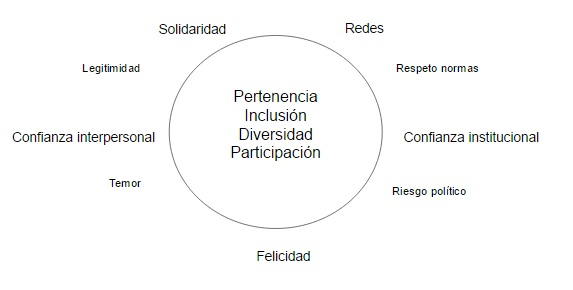
\includegraphics[width=0.75\linewidth]{inputs/images/comun} 

}

\caption{Síntesis de dimensiones}\label{fig:unnamed-chunk-3}
\end{figure}

En un núcleo central, como observamos en la figura {[}figure:dimensiones{]},
se pueden observar las dimensiones que se comparten en mayor medida para
medir la cohesión social en una sociedad por las 5 experiencias
analizadas. Si bien, las experiencias difieren en los indicadores
específicos todas ellas miden de alguna forma la pertenencia, la
inclusión, la diversidad y participación. La pertenencia corresponde a
las identidades o valores que comparten los grupos y sociedades que en
el Social Cohesion Radar es llamada identificación, adhesión a la nación
en ECOsociAL o pertenencia propiamente tal en las experiencias
canadiense y australiana. Por otra parte, la inclusión es otra de las
dimensiones frecuentemente consideradas y que busca medir la forma en
que todos los sujetos son parte de forma equitativa de los beneficios de
la sociedad. Aquí ECOsociAL hace referencia a la percepción de
oportunidades al igual que el Scalon-Monash Index y el Social Cohesion
Radar a la percepción de justicia. Una tercera dimensión hace referencia
que si bien hablamos de un colectivo, este no necesariamente es
homogeneo y que la heterogeneidad no debe afectar la estabilidad o la
cohesividad del grupo. Así, diversos indicadores de multiculturalismo,
reconocimiento y aceptación de la diversidad son incluidos de forma
central por las experiencia analizadas. El índice australiano toma como
un foco central de su monitoreo la condición de los inmigrantes y la
aceptación de la población nativa de los actuales niveles de
inmigración. Asimismo, la experiencia de discriminación es incluida
también por el Scalon-Monash Index. Por otro lado, Social Cohesion Radar
y ECOsociAL incorporan adicionalmente la diversidad religiosa y sexual.
La participación cívica igualmente es una dimensión central en la
medición de cohesión social para la distintas experiencias analizadas.
Esto incluye la participación en organizaciones civíles y participación
propiamente política. Social Cohesion Radar incluye votación en
elecciones, interés en política y el trabajo en asociaciones. Asimismo,
la experiencia australiana lo hace solo con participación política
incluyendo además de votación otras formas de participación como
contacto con representantes, boycot o firma de peticiones. En cambio, el
Mapping Social Cohesion de Canadá incluye la participación electoral y
la participacion en asociaciones voluntarias. En los márgenes de los
elementos centrales, se encuentran otras mediciones de importancia pero
que no son ampliamente abordadas por todas las experiencias revisadas.
Es el caso de la confianza interpersonal y la confianza en las
instituciones. Asimismo, la felicidad o satisfacción con la vida es
considerada por la experiencia canadiense y ECOsociAL. Asimismo, las
redes sociales son caracterizadas a través del contacto con amigos y
sentimiento de soledad. En cuando a la solidaridad se encuentra la
donación de dinero y solidaridad familiar. Estas medidas secundarias
aparecen al menos en dos de todas las experencias incluidas en este
reporte.

Finalmente, se representan algunos de los indicadores que son incluidos
en al menos uno de los monitoreos considerados. Algunas de ellas son la
sensación de temor, el riesgo político o el respeto a las normas
sociales.

De esta forma, este reporte sintetiza 5 experiencias internacionales de
monitoreo de la cohesión social, sirviendo de sustenta conceptual y
operacional para la creación del Observatorio de Cohesión Social en
Chile.

  \bibliography{book.bib,packages.bib,book-ocs.bib}

\end{document}
